\chapter{Planificación}
\label{chap:planificacion}

\lettrine{P}{ara} a planificación dos proxectos é necesaria unha metodoloxía, xeralmente estas seguen unha serie de pasos para o desenvolvemento, neste capítulo explicarase a metodoloxía utilizada e os pasos do proceso de desenvolvemento.

\section{Metodoloxía}
Durante o desenvolvemento deste proxecto seguiuse a metodoloxía de Scrum~\ref{sec:scrum}, aínda que tivemos que adaptala ao noso modo de traballo debido a que está pensada para o desenvolvemento en grupo e non de forma individual como foi o caso neste proxecto. De todas formas é unha metodoloxía perfectamente aplicable xa que basease no aprendizaxe continuo, polo tanto asúmese que o equipo non ten todos os coñecementos ao principio do proxecto e vai ir evolucionando cando se vaia acadando mais experiencia.

\section{Scrum}
~\label{sec:scrum}
~\gls{Scrum} é un proceso de desenvolvemento áxil. Permite un desenvolvemento rápido e por iteracións, permite inspeccionar o software creado e cambiar as preferencias de traballo no lugar dunha planificación e execución completa dende o principio. É un método no que se aplican de maneira regular un conxunto de boas prácticas para traballar de forma colaborativa e obter o mellor resultado posible. Os equipos organizasen entre eles para discutir as funcionalidades e a prioridade destas, deste xeito despois de cada iteración se pode facer unha demostración do produto nese momento. Na figura~\ref{fig:scrum_cycle} pódese ver como é un ciclo dun sprint en Scrum.

\begin{figure}[!ht]
	\caption{Ciclo de sprint en Scrum}
	\centering
	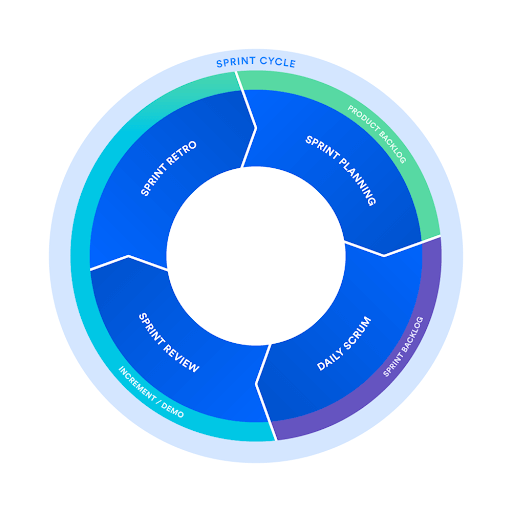
\includegraphics[width=0.7\textwidth]{imaxes/scrum_cycle.png}
	\label{fig:scrum_cycle}
\end{figure}

\subsection{Artefactos Scrum}
Os artefactos son ferramentas que se fabrican para solucionar un problema, en scrum existen tres artefactos que o equipo irá revisando en cada ciclo.
\begin{itemize}
	\item[--] \textbf{Product Backlog:} é a lista principal de traballo que debe realizar o propietario do produto, trátase dunha lista dinámica de funcións, requisitos, melloras e correccións que actúa coma entrada para o sprint backlog. Basicamente é unha lista de tarefas por facer do equipo, estas pódense cambiar de prioridade e se están revisando constantemente xa que é posible que algunhas tarefas deixen de ser necesarias ou os problemas se solucionen de forma diferente, trátase dunha lista dinámica que vai cambiando cos diferentes sprints.
		~\label{scrum:productbacklog}
	\item[--] \textbf{Sprint Backlog:} trátase da lista de elementos, historias de usuario ou correccións de erros seleccionados polo equipo de desenvolvemente para súa implementación no ciclo actual do sprint. Antes de cada sprint, na reunión de planificación, o equipo elixe os elementos nos que vai traballar durante ese sprint. O sprint backlog pode ser flexible e evolucionar durante o sprint.
		~\label{scrum:sprintbacklog}
	\item[--] \textbf{Incremento:} é o obxectivo do sprint, o produto final utilizable ao finalizar este. Dependendo do equipo a finalización do sprint pode ser diferente, cando se lanza un produto ao cliente, se finaliza unha parte dunha versión mais grande~\dots Ao rematar o incremento volve a comezar o ciclo e comeza outro sprint ata que o produto estea finalizado. 
\end{itemize}

\subsection{Protocolos ou eventos de scrum}
Os equipos de scrum realizan periodicamente eventos secuenciais ou reunións. É a parte mais variable xa que dependendo do equipo elimínanse algúns destes eventos, a continuación describiremos todos os protocolos na orde que se executan normalmente.
\begin{itemize}
	\item[--] \textbf{Organización do backlog:} tamén coñecido coma limpeza do backlog, é responsabilidade do propietario do produto, esta persoa encárgase de facer o mantemento da lista do backlog en base aos comentarios dos usuarios e ao equipo de desenvolvemento.
	\item[--] \textbf{Sprint Planning:} esta reunión é dirixida polo scrum master, todo o quipo de desenvolvemento planifica o traballo que se vai realizar durante o sprint actual e decide o obxectivo do sprint. Tamén se fai unha estimación da súa duración e se obtén o Sprint Backlog.
		~\label{scrum:planning}
	\item[--] \textbf{Sprint:} é o período de tempo real que o equipo de scrum traballa de forma conxunta para finalizar un incremento. A duración dun sprint xeralmente é de dúas semanas ou un mes. Canto mais complexo, mais incógnitas haxa, mais corto debería de ser o sprint.
	\item[--] \textbf{Daily Scrum:} trátase dunha reunión diaria duns 15 minutos de duración. O obxectivo é que todos os participantes do equipo estean en sintonía e se adecúen ao obxectivo do sprint cun plan para as seguintes 24 horas. É habitual comezar facendo que cada un dos membros do equipo respondan tres preguntas ¨Qué fixeches onte?¨, ¨Que vas facer hoxe?¨, ¨Que problemas atopaches?¨, é dirixida polo Scrum Master.
		~\label{scrum:daily}
	\item[--] \textbf{Sprint Review:} ao final do sprint, o quipo reúnese nunha sesión informal para ver unha demostración ou inspeccionar o incremento. O equipo de desenvolvemento amosa os elementos do backlog que agora están rematados as partes interesadas e aos compañeiros do equipo, deste xeito poden recibir comentarios ou suxestións.
		~\label{scrum:review}
	\item[--] \textbf{Sprint Retrospective:} o equipo reúnese para documentar e analizar que foi o que funcionou e que non durante o sprint, nun proxecto, nos protocolos etc. A idea é crear un lugar onde o equipo poda centrarse no que saíu ben e que pode mellorarse para a próxima vez.
		~\label{scrum:retrospective}
\end{itemize}

\begin{figure}[hb!]
	\caption{Roles en Scrum}
	\centering
	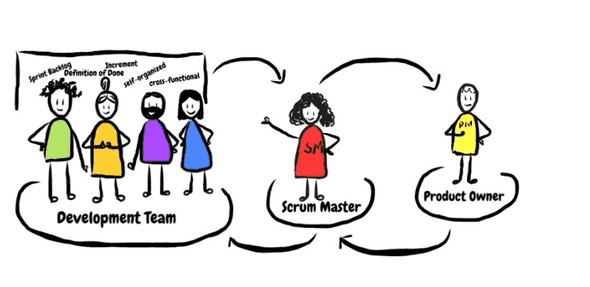
\includegraphics[width=0.9\textwidth]{imaxes/scrum_roles.png}
	\label{fig:scrum_roles}
\end{figure}

\subsection{Roles}
Nesta metodoloxía existen diferentes roles que interpretan distintas persoas, son os seguintes:
\begin{itemize}
	\item[--] \textbf{Product Owner:} son os que mellor coñecen o produto. Están centrados en entender os requisitos empresariais dos clientes e do mercado para despois dar prioridade o traballo que o equipo de enxeñería debe realizara para cumprilos. Crean e xestionan o backlog do produto, asocianse co negocio e co equipo para asegurarse de que todo o mundo entende o traballo, achegan ao equipo directrices claras sobre as funcionalidades que entregar a continuación, tamén deciden cando lanzar o produto. O seu obxectivo é que o produto maximice o seu valor.
	\item[--] \textbf{Scrum Master:} os expertos en scrum son os maiores especialistas en scrum do equipo. Proporcionan formación aos equipos, aos propietarios de produto e a empresa no proceso. Coñecen profundamente o traballo que realiza o equipo e pode axudalo a optimizar a súa transparencia e o fluxo de entrega. Planifican os recursos necesarios para organizar os prazos dos sprints, as reunións rápidas a revisión de sprints e as retrospectivas.
	\item[--] \textbf{Equipo de desenvolvemento:} son os encargados de sacar o traballo adiante. Coñecen as practicas de desenvolvemento sostible. Os equipos mais eficaces teñen unha relación estreita, atópanse na mesma localización e están compostos por entre cinco e sete membros. Os membros do equipo teñen diferentes habilidades, fórmanse entre eles para que ningún quede atrasado. Impulsan o plan en cada sprint, prevén canto traballo creen que poden finalizar ao longo da iteración.
\end{itemize}

\subsection{Scrum no proxecto}
Debido as características do proxecto, algúns dos aspectos da metodoloxía foron adaptados para adecuarse ao proxeto. Scrum contempla esta posibilidade é normal que os equipos adapten o método de traballo as súas necesidades, deste xeito séguese a traballar coa mesma metodoloxía e se obteñen as súas vantaxes sen os inconvenientes que non se poidan subsanar.\smallbreak
Ao realizarse de maneira individual e non dipoñer dun equipo, os roles de Scrum Master e o Equipo de desenvolvemento foron realizados polo alumno, mentres que o de Product Owner polo profesor.\smallbreak
Cada Sprint Planning tivo unha duración de entre dúas semanas e catro, o Daily Scrum foi substituído por un repaso das tarefas realizadas e un diario de traballo e o Sprint Planning realizado de forma individual.\smallbreak
Para a creación do Product Backlog se realizaron reunións ao principio do desenvolvemento para a concreción dos aspectos fundamentais da aplicación, este foi adaptándose co paso do tempo segundo as versións funcionais do produto aproximandose cada vez mais aos requisitos finais como indica scrum.\smallbreak
Os Sprint Backlog foron seleccionados polo alumno segundo as prioridades establecidas inicialmente, tratouse de seguir unha orde lóxica de desenvolvemento de funcionalidades, primeiro as mais básicas que dan xeito ao proxecto e posteriormente as mais específicas que son as que o definen finalmente.\smallbreak
As reunións do Sprint Review coma o Sprint Retrospective foron reducidos debido as características individuais do proxecto.

\section{Planificación inicial}
Unha vez realizado a análise (capítulo~\ref{chap:analise}) se decidiu dividir o traballo en areas, axeitando estas a planificación da metodoloxía:
\begin{itemize}
	\item \textbf{Configuración inicial do proxecto:} Esta primeira fase incluíu a recolección de información sobre as ferramentas a utilizar para a posta en marcha do proxecto, o estudo de diferentes métodos para a implementación das bases do proxeto e a configuración do entorno de desenvolvemento, tamén se fixo a inicialización dos frameworks.
	\item \textbf{Desenvolvemento do backend:} Posteriormente, creouse a lóxica do backend, desenvolveuse a API propia, crearonse as peticións necesarias da aplicación ao API de Spotify e por último a configuración da xestión de usuarios no backend.
	\item \textbf{Creación da base de datos:} Na terceira fase, fíxose o deseño da base de datos, modificouse o modelo de usuarios de Django e se crearon o resto dos modelos. Tamén se estudaron as posibilidades de almacenamento de datos na parte do frontend.
	\item \textbf{Xeración do espazo web:} Antes da implementación do frontend fíxose un deseño do entorno web en mockups~\ref{fig:mockups}, posteriormente se trasladou este deseño ao espazo web creando as diferentes páxinas.
	\item \textbf{Conexión do frontend co backend:} Por último conectouse completamente o backend co frontend, implementaronse as vistas e controladores do frontend, creouse a conexión con \acrfull{JWT} para a securización dos datos e completouse a administración de usuarios.
\end{itemize}

\begin{figure}[hp!]
	\caption{Mockups do frontend}
	\label{fig:mockups}
	\centering
	\begin{subfigure}[c]{1\textwidth}
		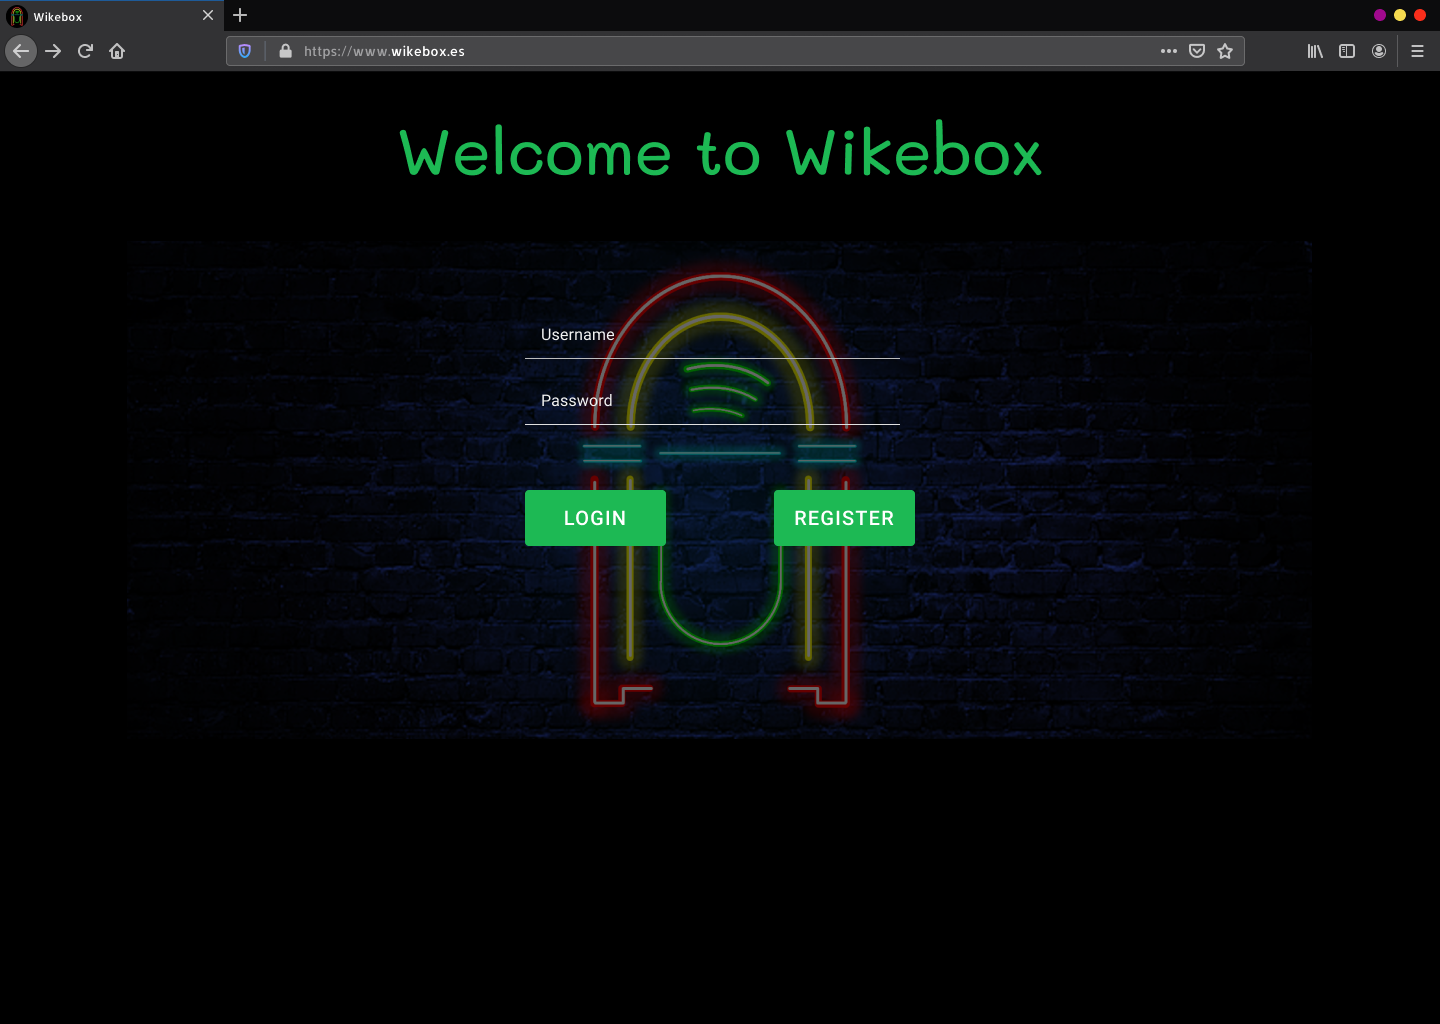
\includegraphics[width=\textwidth]{imaxes/Login.png}
		\caption{Mockup vista de login}
		\label{fig:mockup_login}
	\end{subfigure}
	\begin{subfigure}[c]{1\textwidth}
		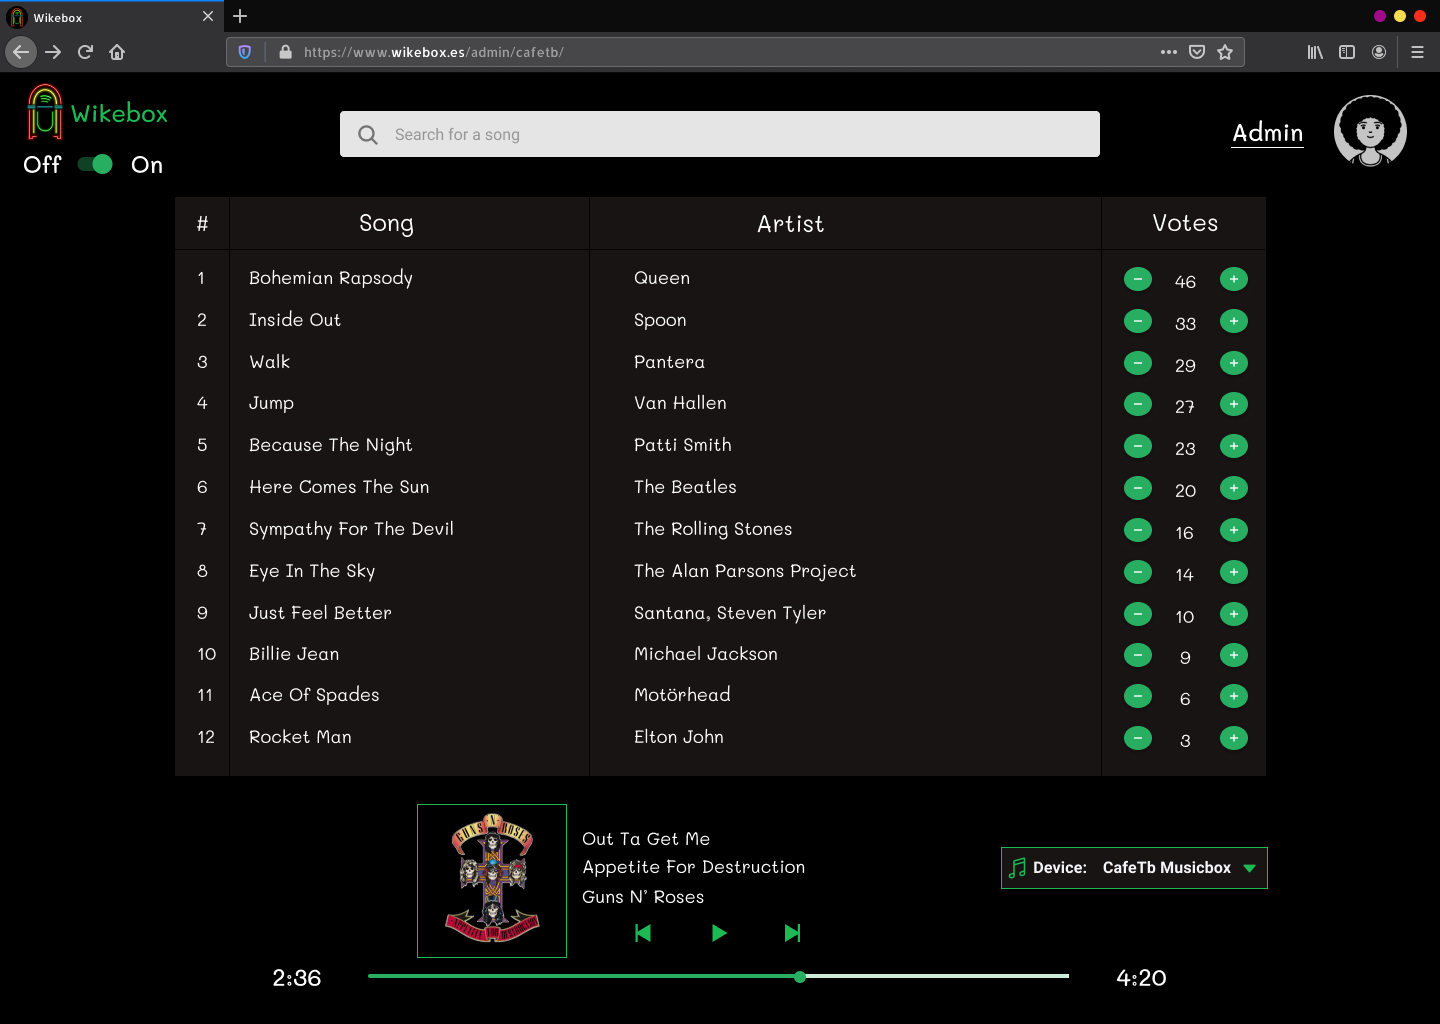
\includegraphics[width=\textwidth]{imaxes/Admin_home.png}
		\caption{Mockup vista do admin}
		\label{fig:mockup_admin_home}
	\end{subfigure}
\end{figure}%
\begin{figure}[hp!]
	\ContinuedFloat
	\centering
	\begin{subfigure}[c]{1\textwidth}
		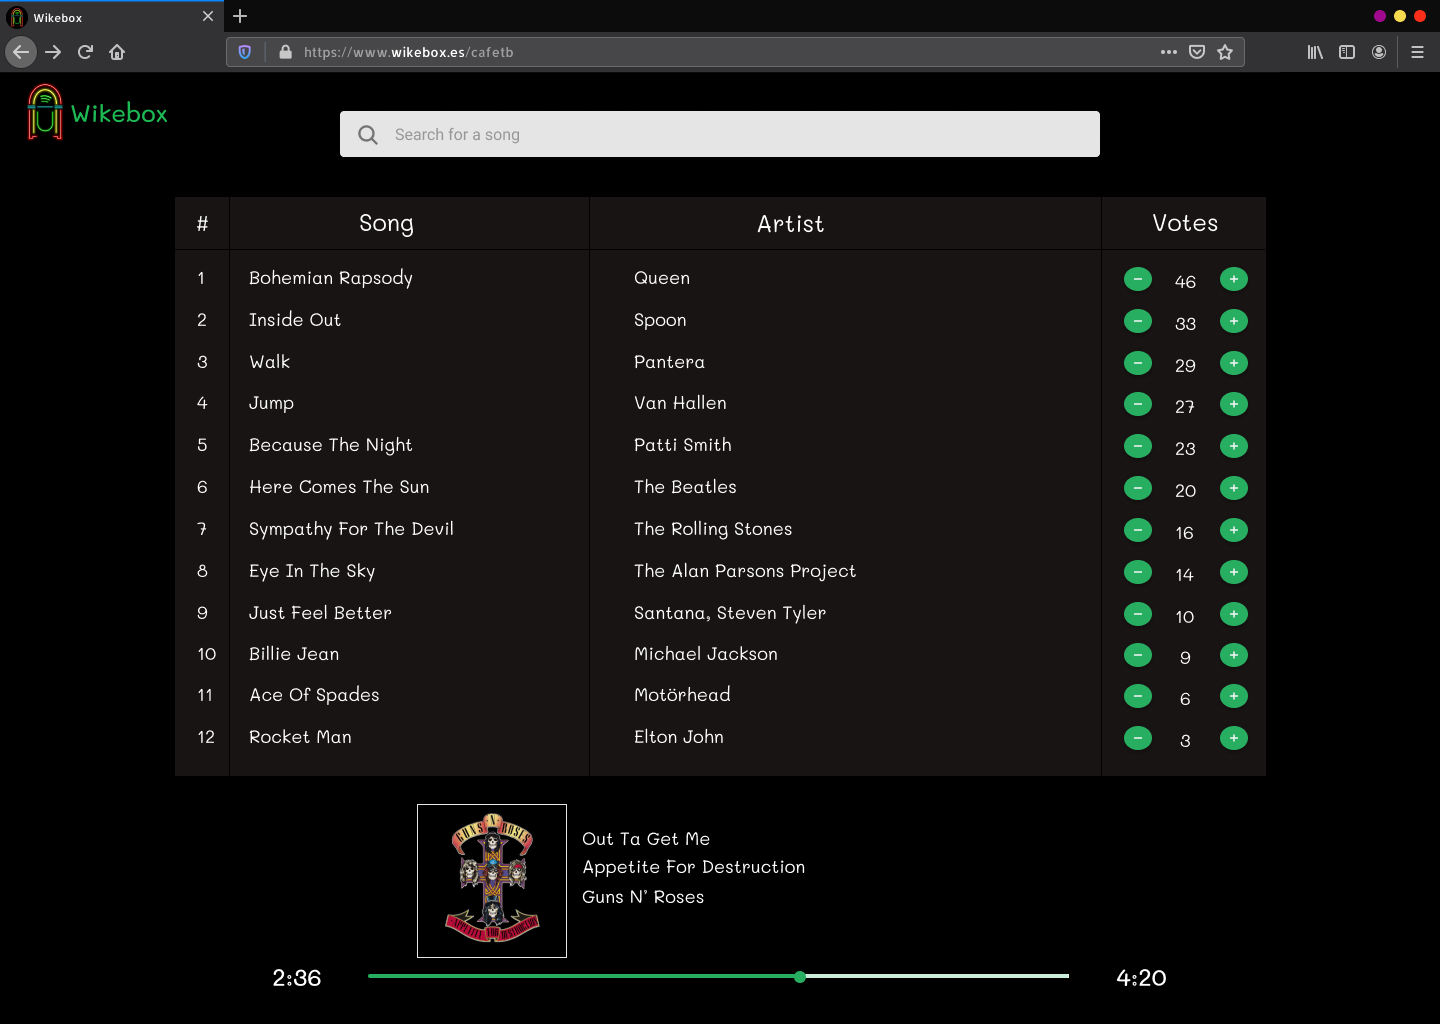
\includegraphics[width=\textwidth]{imaxes/User.png}
		\caption{Mockup vista de usuario}
		\label{fig:mockup_usuario}
	\end{subfigure}
	\begin{subfigure}[c]{1\textwidth}
		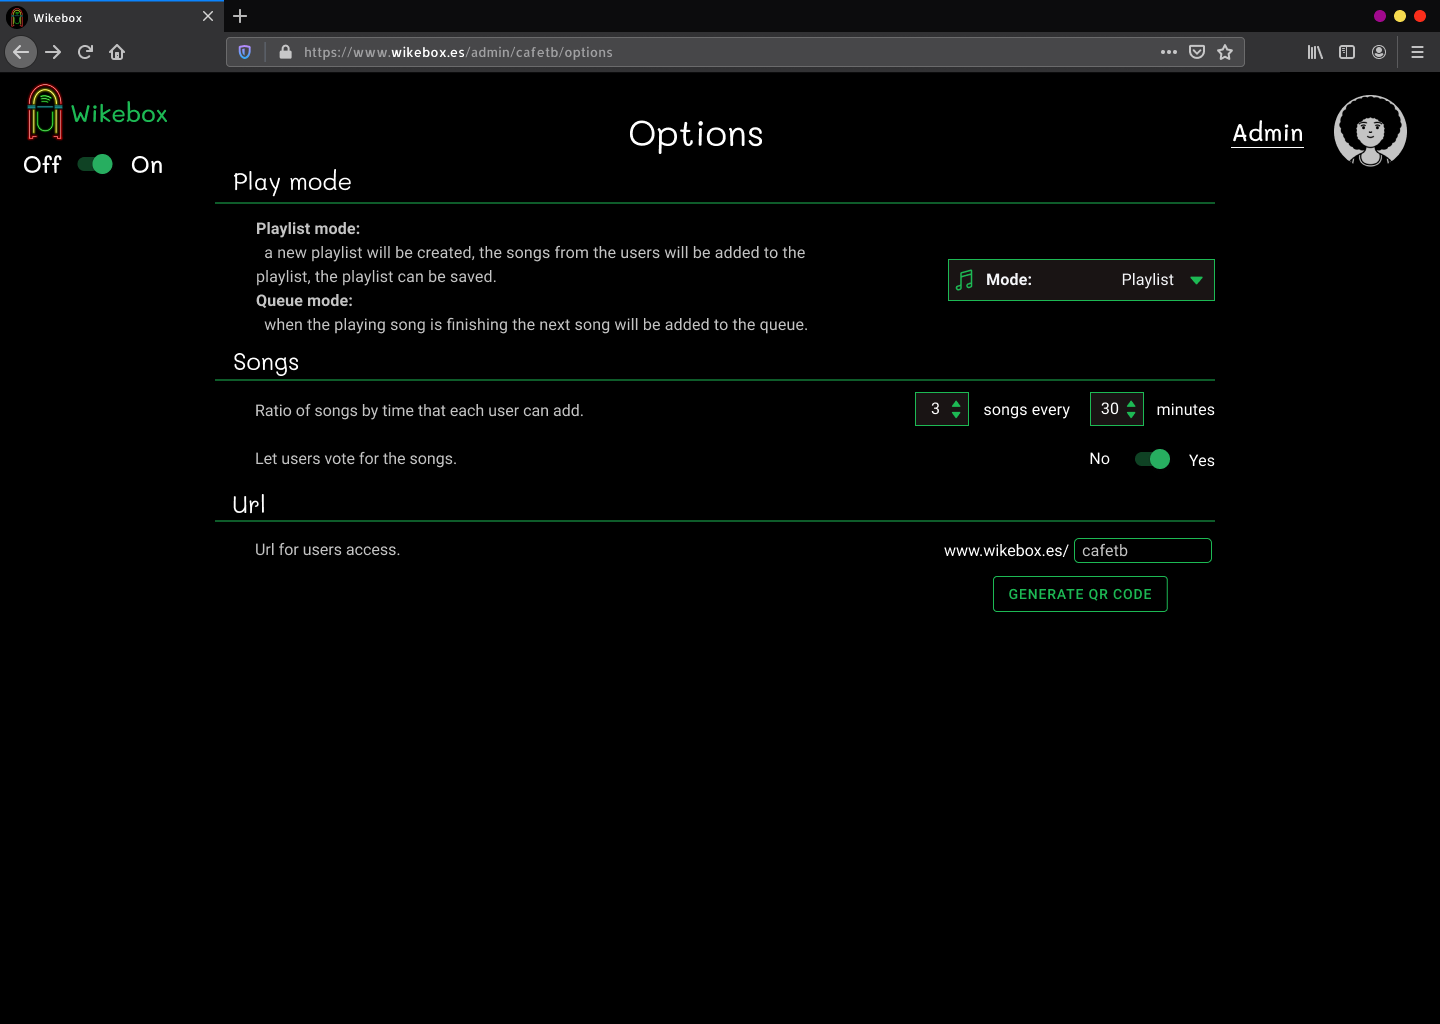
\includegraphics[width=\textwidth]{imaxes/Admin_options.png}
		\caption{Mockup opcións do admin}
		\label{fig:mockup_admin_options}
	\end{subfigure}
\end{figure}

\section{Adaptación da planificación a Scrum}
O desenvolvemento do proxecto se dividiu en 5 fases ou sprints, as cales tiveron unha duración de entre 3 e 5 semanas dependendo da complexidade, a metodoloxía foi adaptada a natureza do proxeto. Se realizou un Sprint Planning~\ref{scrum:planning} ao principio de cada fase onde se obtivo o Sprint Backlog~\ref{scrum:sprintbacklog} e ao finalizar cada unha se fixo o Sprint Review~\ref{scrum:review} para a creación do seguinte Sprint Backlog. Durante a realización do proxecto, tamén se levou un diario de traballo, no que se levaba rexistro das tarefas realizadas, isto tamén facilitou a organización.

\subsection{Primeiro sprint}
No primeiro sprint levouse a cabo a implementación da primeira fase, creouse o Product Backlog~\ref{scrum:productbacklog} baseado nos requisitos funcionais. Posteriormente estableceuse o espazo de traballo, configurouse o editor NeoVim cunha selección de plugins adaptados aos frameworks elixidos e ao desenvolvemento, tamén se configurou o repositorio de GitHub. Neste sprint tamén fíxose a inicialización de ambos frameworks e fixéronse probas de funcionamento con Ionic xa que se trataba dun framework novo para o desenvolvedor, rexistrouse a aplicación en Spotify o que permite facer peticións a seu API. Fíxose unha procura de documentación inicial para orientar o proxecto as mellores ferramentas dispoñibles na actualidade.

\subsection{Segundo sprint}
Nesta fase implementouse o backend, creouse unha aplicación de Django que fai de API, para a comunicación entre os frameworks. Xeneraronse as peticións ao API de Spotify coa axuda da libraría \textit{Spotipy}, tanto as cancións, as procuras coma a obtención dos datos do que se está a reproducir nese intre. Tamén se fixeron as modificacións necesarias para usar o sistema de xestión de usuarios de Django, aínda que tería que ser modificado posteriormente.\smallbreak
Ao finalizar o Sprint comprobouse coa aplicación de Postman~\ref{sec:postman} que o backend respondía as peticións e era capaz de facer modificacións na reprodución de música a través do API.

\subsection{Terceiro sprint}
Neste sprint deseñouse a base de datos, fíxose un modelo relacional que se trasladou a aplicación, crearonse os modelos de datos en Django para gardar as sesións, as listas de reprodución das sesións e as cancións que están a soar. Modificouse o modelo xa preestablecido de usuarios en Django para engadir datos de interese coma a sesión a que pertence o usuario e retiráronse outros campos coma o enderezo electrónico, na figura~\ref{fig:database} podemos ver a súa estrutura. Tamén buscáronse as diferentes alternativas para o almacenamento de datos no frontend.\smallbreak
No Sprint Review comprobouse que era posible o almacenamento dos datos obtidos da plataforma de música e tamén era posible a súa lectura.

\subsection{Cuarto sprint}
Para o cuarto sprint se planificou o deseño do frontend baseado nos mockups realizados, crearonse as páxinas adaptándoas o máximo posible ao deseño. Implementouse o servizo no frontend encargado de facer as peticións ao backend. Crearonse as peticións necesarias para a obtención dos datos e se creou a xestión de usuarios tendo en conta os permisos de acceso tanto na parte do frontend coma do backend permitindo tan só as accións necesarias.\smallbreak
Para rematar o sprint comprobouse que o servidor de Ionic era capaz de amosar as diferentes páxinas web e que funcionaban as características implementadas ata o momento.

\subsection{Quinto sprint}
O último sprint foi o mais longo debido a dificultade de securizar o sistema, fíxose mediante \acrshort{JWT} para a xestión de tokens para os usuarios. Estudáronse outros métodos para facer dita conexión, pero se concluíu que a autenticación con \acrshort{JWT} era a mais segura e útil no noso caso. Implementouse un middlware capaz de interceptar as petición e engadir os tokens de acceso, tamén coa posibilidade de renovalos cando é necesario. Por último crearonse as peticións que restaban para a comunicación co backend.\smallbreak
Ao final o Sprint Review comprobouse que a aplicación era funcional e segura, para os usuarios rexistrados non presenta ningunha modificación pero os usuarios non rexistrados non teñen capacidade de facer peticións ao API.

\section{Custos do proxecto}
A medición dos custos se fai contemplando entre diferentes categorías os custos técnicos, referentes equipamento hardware e software necesario, custos de servizos, referente aos servizos contratados e custos en recursos humanos. Debido a que non foi necesaria a compra de ningún equipamento nin o aluguer de ningún servidor e tampouco foi necesaria a adquisición de ningún software xa que o utilizado foi gratuíto conclúese que os custos técnicos son nulos, non así os outros.\medbreak
Para dispor do funcionamento completo da API de Spotify é necesaria a subscrición ao seu servizo \textit{premium} o que ademais ofrece outras vantaxes. Na táboa~\ref{tab:spotify_plans} pódese observar os custos dos diferentes plans ofertados, no noso caso utilizouse unha subscrición familiar que resulta nun montante de 2,67 € mensuais e aproximadamente 14 € durante a duración do proxecto.\medbreak
Para o cálculo do custo dos recursos humanos é necesario coñecer o tempo invertido, desafortunadamente non acadouse a precisión desexada e fíxose unha estimación que podemos observar na táboa~\ref{tab:custos_humanos}. Do mesmo xeito non é doado impoñer un custo por hora traballada xa que nun proxecto con diferentes recursos humanos existen custos distintos para cada un dos recursos. Decidiuse un prezo de 20 € por hora traballada para realización dos cálculos.\medbreak
Na seguinte táboa~\ref{tab:custos_proxecto} podemos ver o custo total aproximado do proxecto.

\begin{table}[hp]
	\caption{Custos do proxecto}
	\label{tab:custos_proxecto}
	\begin{center}
		\begin{tabular}{| l | l |}
			\hline
			Concepto & Custo\\ \hline
			Spotify premium & 14 € \\
			Recursos humanos & 9200 € \\
			{\textbf{Subtotal}} & {\textbf{9214 €}} \\ 
			IVE (21 \%) & 1934,34 € \\
			{\textbf{Total}} & {\textbf{11148,94 €}} \\ \hline
		\end{tabular}
	\end{center}
\end{table}

\begin{table}[hp]
	\caption{Tempo empregado no proxecto}
	\label{tab:custos_humanos}
	\begin{center}
		\begin{tabular}{| l | l |}
			\hline
			Tarefa & Tempo en horas\\ \hline
			Documentación & 80 \\
			Desenvolvemento do backend & 100 \\
			Desenvolvemento do frontend & 100 \\
		    Conexión e securización & 150 \\
			Probas & 30\\
			{\textbf{Total}} & {\textbf{460}} \\ \hline
		\end{tabular}
	\end{center}
\end{table}
